% !TEX root = ../thesis.tex

% set counter to n-1:
\setcounter{chapter}{0}

\chapter{Introduction}\label{chap:intro}
\section{Action Recognition}
Video based action recognition finds its usage in a broad range of practical applications such as surveillance, video analysis and retrieval as well as human computer interaction. In the recent years, evidently increasing research effort has been devoted in this topic. However, despite the intense research, it remains one of the unconquered fields in computer vision.

The two major milestones are marked with the development of a series of trajectory based feature extractor \cite{wang2011action,wang2013action} and the success application of deep neural network in action recognition \cite{simonyan2014two}. 
The former, typically used in the standard Bag of Visual Words (BoVW) pipeline together with advanced encoding method \cite{perronnin2010improving, peng2014action}, is broadly used as benchmark for later methods. 
Meanwhile the latter, the first Convolutional Neural Network (CNN) \cite{lecun1989backpropagation} based approach that yielded competitive performance, stimulated many valuable follow-up proposals with various focuses oriented on improvements for deployment of deep neural network in action recognition \cite{wang2015temporal,xiong2015recognize}.

However, as video datasets become more and more challenging, the performance of CNN based methods seem to have reached a bottleneck. 
In particular, as video clips gets more realistic and the temporal trimming more fuzzy, the definition of "action" demands a second thought. 

On one hand, an action is a series of events connected in time, recognizing an action often requires consideration of temporal evolution. 
The original CNN tackles this issue by applying a simple temporal pooling on the frame-wise classification results, which becomes an apparent weakness when dealing with long untrimmed video sequences. 
In order to tackle this drawback, 3D-CNN \cite{ji20133d} as well as LSTM (Long Short Term Memory) Models \cite{donahue2015long,yue2015beyond} have been opted to emphasize the evolvement in time. 
However, given the complexity of their architectures, the performance yielded by such approaches are harshly jeopardized by the inadequacy of available datasets.

On the other hand, the recognition of an action in video can be seen as an interplay of recognizing different components of an event. 
In fact, for many action categories one does not even need any temporal evolution to classify them; as is shown in \autoref{fig:singleframe}, one can easily classify the whole video sequence given the composition of objects or scene in a single frame. 
As a matter of fact, this concept has already been widely implemented and intensely optimised in low-level features, primarily by applying various fusion techniques \cite{peng2014bag} on descriptors from different cues such as Histogram of Gradients (HOG) \cite{laptev2008learning} for appearance cue and Motion Boundary Histogram (MBH) \cite{wang2013action} for motion cue. However on semantic level this field still remains scarce. 

\begin{figure}
\centering
\begin{subfigure}{0.30\textwidth}
	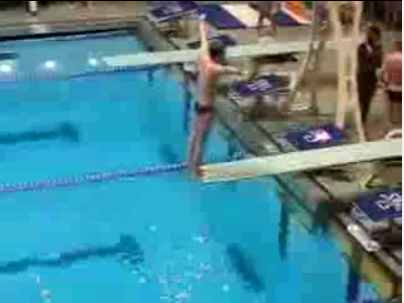
\includegraphics[height=3cm, width=4cm, keepaspectratio=false]{figures/scene_domi0.png}
\caption{Scene}\label{fig:scenedomi}
\end{subfigure}
\begin{subfigure}{0.30\textwidth}
	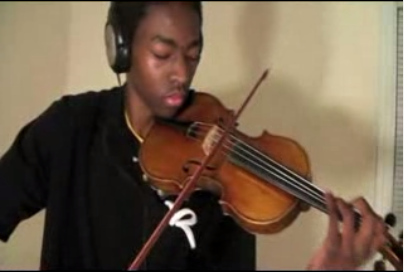
\includegraphics[height=3cm, width=4cm,]{figures/obj_domi0.png}
\caption{Object}\label{fig:objdomi}
\end{subfigure}
\caption[Scene and object centric videos]{Sample frames from UCF101 dataset, where perceptually the appearance of scene or objects is sufficient for correct recognition of an action class.}\label{fig:singleframe}
\end{figure}

\begin{figure}
\begin{subfigure}{0.5\linewidth}
\begin{tikzpicture}[nodes={font=\footnotesize,anchor=center}]
\node[inner sep=0pt] (h1) at (0,0)
    {\includegraphics[width=.3\columnwidth]{figures/babycrawling.png}};
\node[below] at (h1.south){BabyCrawling};
\node[right=0pt of h1,inner sep=0pt] (h2)
    {\includegraphics[width=.3\columnwidth]{figures/handstandwalking.png}};
\node[below] at (h2.south){Handstand};
\node[right=0pt of h2, inner sep=0pt] (h3)
    {\includegraphics[width=.3\columnwidth]{figures/pushup.png}};
\node[below] at (h3.south){PushUp};
\end{tikzpicture}
\caption{Body Motion Only}
\end{subfigure}
\begin{subfigure}{0.5\linewidth}
\begin{tikzpicture}[nodes={font=\footnotesize,anchor=center}]
\node[inner sep=0pt] (h1) at (0,0)
    {\includegraphics[width=.3\columnwidth]{figures/pizzatossing.png}};
\node[below] at (h1.south){PizzaTossing};
\node[right=0pt of h1,inner sep=0pt] (h2)
    {\includegraphics[width=.3\columnwidth]{figures/playingviolin.png}};
\node[below] at (h2.south){PlayingViolin};
\node[right=0pt of h2, inner sep=0pt] (h3)
    {\includegraphics[width=.3\columnwidth]{figures/archery.png}};
\node[below] at (h3.south){Archery};
\end{tikzpicture}
\caption{Human Object Interaction}
\end{subfigure}
\begin{subfigure}{0.5\linewidth}
\begin{tikzpicture}[nodes={font=\footnotesize,anchor=center}]
\node[inner sep=0pt] (h1) at (0,0)
    {\includegraphics[width=.3\columnwidth]{figures/frontcrawl.png}};
\node[below] at (h1.south){frontcrawl};
\node[right=0pt of h1,inner sep=0pt] (h2)
    {\includegraphics[width=.3\columnwidth]{figures/surfing.png}};
\node[below] at (h2.south){Surfing};
\node[draw=blue, right=0pt of h2, inner sep=0pt] (h3)
    {\includegraphics[width=.3\columnwidth]{figures/skydiving.png}};
\node[below] at (h3.south){SkyDiving};
\end{tikzpicture}
\caption{Body Motion in Specific Scene}
\end{subfigure}
\begin{subfigure}{0.5\linewidth}
\begin{tikzpicture}[nodes={font=\footnotesize,anchor=center}]
\node[inner sep=0pt] (h1) at (0,0)
    {\includegraphics[width=.3\columnwidth]{figures/bowling.png}};
\node[below] at (h1.south){Archery};
\node[right=0pt of h1,inner sep=0pt] (h2)
    {\includegraphics[width=.3\columnwidth]{figures/balancebeam.png}};
\node[below] at (h2.south){BalanceBeam};
\node[right=0pt of h2, inner sep=0pt] (h3)
    {\includegraphics[width=.3\columnwidth]{figures/writingonboard.png}};
\node[below] at (h3.south){WriteOnBoard};
\end{tikzpicture}
\caption{Human Object Interaction in Specific Scene}
\end{subfigure}
\caption[Categorization of Actions according to Semantic Composition]{Action classes can be grouped into four types: (1) body motion only, (2) human object interaction, (3) human in specific scene, and (4) human object interaction in specific. Classifying each of these categories may require a diverse emphasis on the semantic cues, like human body (red box), interacting objects (green box), and global context (blue box).}\label{fig:categories}
\end{figure}
\section{Objective, Challenge and Contribution}
As aforementioned, the definition of an action is manifold rather than straightforward. Often a successful recognition process involves diverse factors. 
Inspired by natural human perceptual procedure, we define three most relevant cues in action recognition, namely: the action performer (person) including his appearance and motion, objects in case of human-objection interaction and the actual scene where the action takes place. 
In most cases, person should be the most decisive cue, but under certain circumstances, the other two cues could be dominating or even essential. 
Current CNN-based action recognition methods mostly use the whole frame as input. Consequently, the network is expected to infer the internal relations automatically and ideally learn to shift its attention to the most informative cue.

Regardless of CNN's great performance in the task of action recognition, it is unclear: 
\begin{itemize}
\item what the network has actually learned
\item whether it's able to abstract the different semantic cues and internalize their relations with respect to the target action
\end{itemize}

In order to answer these questions, we divide the existing action classes into four sub-categories, namely 
\begin{enumerate}
\item Body Motion Only (referred as "\textit{P}"), where the action is defined solely by the motion and appearance of the involving person;
\item Human-Object Interaction (referred "\textit{P+O}"), where the action involves a specific object;
\item Body Motion in specific Scene (referred as "\textit{P+S}"), where the action takes place in a discriminative environment; 
\item Human Object Interaction in specific Scene (referred "\textit{P+O+S}"), where the action involves both a particular object and a distinct environment.
\end{enumerate} 
Examples of this categorization on UCF101\cite{soomro2012ucf101} dataset is shown in \autoref{fig:categories}. (for the complete categorization results of dataset UCF101, please refer to \autoref{tab:101categories} in appendix).
This categorization reflects the relative relevance of the three semantic cues in a given action class and will be used as a guideline for analysis through the thesis.

Using this categorization, we evaluated the per category performance on UCF101 and observed significantly inferior test accuracies in categories \textit{P} (see \autoref{tab:worstucf}).
This indicates that under current datasets, deep neural networks are not yet able to abstract high level semantic structures and is often perturbed by ambiguous information.

\begin{table}
\centering
\begin{tabular}{|p{\widthof{class ratio with $ <\%50 $ acc. }}|cccc|}
\hline
& P & P+O & P+S & P+O+S \\ \hline
class ratio with $ <\%50 $ acc. & $ \frac{4}{21} $ & $ \frac{3}{25} $ & $ \frac{3}{28} $ & $ \frac{1}{27} $\\ 
mean Acc. &$ 64.08\% $ & $ 81.32\% $& $ 81.66\% $ & $ 88.40\% $\\ \hline 
\end{tabular}
\caption[Evaluation of worst performing classes w.r.t semantic composition]{UCF action classes with test accuracy lower than $ <\%50 $ (split 1).} \label{tab:worstucf}
\end{table}

This observation motivated us to explicitly incorporate semantic structure into the CNN architecture.

One possible and probably the most straightforward approach is to train separate classifiers for each cue and fuse a final result by applying various late or early fusion methods. 
While this may indeed yield better result in terms of accuracy, it does so at the cost of generability and scalability, thus certainly not a long-term solution. 
In contrary we aim to keep our system as concise, general and computational efficient as possible.

Specifically, we propose an integrated deep neural network framework, which combines various detection results (i.e. semantic cues) into a two-stream action recognition pipeline. 
We use the recently proposed Faster-RCNN \cite{ren2015faster} as human and common object detector and adapt them to the video domain by leveraging temporal constraints among a sequence of detection results.
These temporally coherent detection results provide semantic information about the activities portrait in the videos, such as the locations of a person and the relations of person and objects over time. 
We incorporate these semantic cues (detection results) into proposed action recognition pipeline, where detected bounding boxes guide the localization of salient regions in the video stream and enable CNNs to select discriminative features with ROI (Region Of Interest) pooling \cite{girshick2015fast}. 
In order to fuse semantic channels in an optimal fashion, we propose and evaluate different fusion methods and training strategies to optimize the weights of our deep models.
We empirically study the effect of different settings and make recommendations for the best choice.

In summary the contribution of this thesis includes:
\begin{enumerate}
	\item We proposed a CNN model on weakly annotated video to encode the semantic decomposition of in action cognitive process into the three cues, namely person, interacting objects and scene. We achieve state-of-art performance on UCF101 dataset. Meanwhile by utilizing the complementary properties of the cues, we increase the robustness of our model.
	\item In addition, we systematically study the effect of incorporating semantic cues on the recognition performance for different types of action classes as defined previously, and try to provide some insights for building more reasonable action benchmarks and robust recognition algorithms.
\end{enumerate}

\section{Thesis Outline}
\begin{itemize}
\item In \autoref{chap:relatedwork} we start with an detailed overview on action recognition with particular focus on the previous approaches concerning the utilization and leverage of semantic cues.
\item \autoref{chap:model} provides an overall introduction to our approach.
\item The specific implementation details concerning training and testing settings will be summarized in \autoref{chap:setup}.
\item Finally in \autoref{chap:result}, we give a comprehensive analysis based on our empirical study.
\end{itemize}

